\clearpage
\setcounter{page}{1}

\section{绪论}
\label{sec:intro}

光纤传感器的出现让实时确定物体的形态成为了一个很有前景的研究方向\cite{recent-dev-in-foss}。
光纤形变传感器(Fiber Optic Shape Sensors, FOSS)被设计用于定向应变测量,例如,
FOSS可以由三芯光纤布拉格光栅(Fiber Bragg Grating, FBG)传感器组成,
该传感器测量应变以进行对象的多维曲率计算,可以在计算机模型中用于重建对象的二维和三维形状。
然而,尚未有针对如何构建通用三维可视化软件方面的研究。

本章主要讨论\nameref{sec:ss},并提出一种三维可视化软件的架构。

\subsection{形变传感器的研究方向及进展}
\label{sec:ss}

形变传感器主要分为两大类,一类是传统形变传感器(Conventional Shape Sensors, CSS),
另一类是光纤形变传感器(Fiber Optic Shape Sensors, FOSS), 
其中传统形变传感器又分为非接触式和接触式两种。

非接触式传感器包括视觉系统传感器(如相机)、
无线电监测与测距(Radio Detection and Ranging, RaDAR)
或光监测与测距(Light Detection and Ranging, LiDAR)传感器,
这些传感器的性能与正确性受环境温度和污染干扰很大。

随着传感器的需求场景越来越多且复杂,非接触传感系统越来越局限,
对小型且灵活的接触式传感器的需求也就越来越大。
接触式传感器可以直接连接到物体上随其移动,
并将位置转换为光、电信号以感测形状、曲率、弯曲和扭曲。

接触式CSS主要分为电阻压力传感器、电光传感器和微机电系统(Micro-Electo-Mechanical System, MEMS)传感器。
其中电阻压力传感器基于压敏电阻;
电光传感器基于陀螺仪、加速度计等电子传感器和光传感器组成的传感网络;
MEMS传感器基于微机电系统。它们各自的优缺点和应用场景对比如表~\ref{table:css}所示。

\begin{table}[h]\footnotesize
\caption{三种接触式CSS对比}
\label{table:css}
\begin{center}
\begin{tabular}{p{0.16\textwidth}p{0.16\textwidth}p{0.24\textwidth}p{0.24\textwidth}}
\toprule
\textbf{传感器类别} & \textbf{优点} &\textbf{缺点} & \textbf{应用场景}\\

\midrule

电阻压力传感器 &
低成本;与其它电器件相兼容& 
不够精准;尺寸重量过大;复杂且接线繁琐&
消费级电子产品,如游戏用压感器、穿戴式心率检测仪。
\\
\\

电光传感器 &
易于大规模生产;与Arduinos等价格低廉的微电子设备兼容&
要求传感器周围有自由空间,以便光学传感器能够正常工作;无法保证精度 &
医疗运动和预防伤害,如人体肌肉脊椎形状传感。
\\
\\

MEMS传感器 & 
精度高;功耗小;可靠性高& 
难以定制;笨重;低柔韧性;昂贵&
工业场景,如钻井、海床监控、精加工等\\
\bottomrule
\end{tabular}
\end{center}
\end{table}

\FloatBarrier
\subsubsection{光纤形变传感器}
通常,FOSS与CSS相比具有许多明显而实用的优点,例如:
\begin{itemize}
\setlength{\topsep}{0pt}
\setlength{\itemsep}{0pt}
\setlength{\parsep}{0pt}
\setlength{\parskip}{0pt}
\item FOSS可以仅由一个远程询问器单元进行监控,而无需布线和连接许多传感器。
\item 传感元件(如光纤光栅)不需要电力,抗电磁干扰能力强。
\item 小尺寸的光纤(直径在100μm和2mm之间)可以嵌入非常薄的物体中。
\end{itemize}

\begin{table}\footnotesize
\caption{FOSS的发展趋势\cite{recent-dev-in-foss}}
\label{table:foss}
\begin{center}
\tabcolsep=0.10cm
\begin{tabular}{p{0.16\textwidth}cp{0.64\textwidth}}
\toprule
\textbf{进展} & \textbf{年份} & \makebox[5cm][c]{\textbf{简介}}\\

\midrule

弯曲传感器 & \textasciitilde 1980 & 确定了三种主要的早期弯曲感测方法。它们分别是:
通过正常光纤传输的功率变化感测;
通过配备了弯曲调制器的光纤传输功率变化感测;
通过同一包层中并行核心之间的串扰而导致的传输功率变化感测。
\\
\\
定向弯曲传感器 & \textasciitilde 1990 & 通过使用多根单独的光纤和多芯光纤,可以检测光纤弯曲方向。
其采用了多种技术,如单个的FBG、宏弯曲调制器、多芯光子晶体光纤模场变化和弯曲引起的芯串扰。
\\
\\
分布式弯曲传感 & \textasciitilde 1996 & 通过多路复用,光纤能够通过FBG在多个位置检测应变。 
最初,只有波分和时分多路复用用于光纤形状感测,这限制了传感器的数量和最小的弯曲半径。
\\
\\
第一款商用3D光纤形变传感(ShapeTape)& \textasciitilde 1999 & ShapeTape是最早用于计算物体形状和表面的光纤3D测量设备之一。 
它是在1990年代基于光纤压力传感器开发的。 
由于价格高,范围、灵活性和准确性都很有限,ShapeTape在商业上并不成功。
\\
\\
基础光纤形变传感 & \textasciitilde 2000 & 通过多路复用检测多个位置处的弯曲,为三维形状感测提供了机会。
三个或更多芯的光纤提供了在多个位置检测方向应变的能力,从而可以重构空间中的光缆形状。
\\
\\
分布式光纤形变传感 & \textasciitilde 2004 & 在多个磁芯上数千个应变位置的检测使连续光栅感测三维形状成为可能,
从而消除了先前形状感测技术的离散性质。 
光频域反射计(Optical Frequency Domain Reflectometry, OFDR)可以利用普通光纤和连续光栅光纤中的瑞利反向散射光进行形状感测。
\\
\\
用于工业和医疗机器人的光纤形变传感 & \textasciitilde 2006 & 各种专利的出现促使着工业和医疗器械中FOSS的使用,
这是工业界第一次在实际应用中对FOSS表现出兴趣。
\\
\\
螺旋光纤布拉格光栅传感器 & \textasciitilde 2008 & 多芯光纤中使用螺旋FBG进行扭曲和弯曲测量的第一个演示,
这为如何基于FOSS实现完整的3D重建提供了改进思路。
\\
\\
光纤形变传感可视化 & \textasciitilde 2009 & 随着返回信号愈发复杂,渲染出使用光纤形状感测的电缆变得更具挑战性。
自2009年以来,越来越多的论文和专利概述了实时渲染FOSS输出的各种方法。
\\
\\
基于光纤形变传感器的力传感 & \textasciitilde 2013 & 使用光纤形状感测电缆测量力不仅可以检测光纤的位置,
还可以检测该点的力。这些论文和专利自2013年以来由医疗器械公司出版,
为多功能形状传感器开辟了道路。
\\
\\
基于多芯光纤和分布式FOSS的分布式布里渊散射 & \textasciitilde 2016 & 首次演示了通过多芯光纤(Multi-Core Fiber, MCF)
中偏心纤芯的布里渊频移来测量长光纤(1km)中的曲率,为远程形状感测带来了新的可能性。
\\
\\
螺旋多芯光纤中的连续光栅 & \textasciitilde 2017 & 关于连续光栅多芯光纤的研究有了新的进展。
复合多芯光纤的商业可用性对于开发高分辨率和分布式FOSS来说至关重要。
\\
\bottomrule
\end{tabular}
\end{center}
\end{table}

FOSS的发展趋势总结如表~\ref{table:foss}所示。
在1980年代左右,已有研究者考虑使用光纤开发弯曲传感器\cite{meltz_fiber_1981,schiffner_sensing_1984,Lagakos:87},
并在1990年代初开始研究定向弯曲测量\cite{clements_fiber_2005,danisch_fiber_1994,greenaway_optical_1999,greenaway_optical_2002,10.1117/12.2302270}。

1996年Davis等研究者基于FBG和波分复用(WDM)技术开发了一种可测量光纤的多个位置应变和弯曲的FOSS\cite{Davis_1996}。 
2001年Chen和Sirkis提出了分布式弯曲感测系统的总体思路,这种系统具有弯曲和扭曲测量功能,使得重建物体完整的三维形状成为可能\cite{chen_method_2001}。

1999年Ravin等研究者开发了一种新的光纤二维弯曲扭曲感应条,商业上被称为“ShapeTape”\cite{ShapeTape}。
ShapeTape利用一种称为“Kinotex”的压敏光纤产品来检测胶带不同区域上的压力并在计算机屏幕上显示形状。
因为价格高昂和测量精度、范围、灵活度等方面的限制,ShapeTape没有取得很大成果。

在2000年初,有研究者提出多芯光纤可利用FBG的相位和应变变化实现高精度曲率感测\cite{flockhart_differential_2006,Araujo:02}。
但使用WDM进行形状感测的缺点是可利用的FBG数量受到限制,从而限制了对更长或更灵活对象的测量。

随着计算能力的提高和分布式光纤传感技术的发展,2004年Askins等研究者提出利用光频域反射法(OFDR),
使用数百至数千个FBG或光纤段在数百米长的单根光纤上以毫米分辨率测量反向散射,可实现分布式高分辨率FOSS\cite{10.1117/12.566653}。
2008年他们又提出一种利用螺旋多芯光纤进行弯曲和扭曲传感的方法,此后该方法成为多种FOSS的核心\cite{4528404}。

2009年开始,越来越多的论文和专利概述了实时渲染FOSS输出的各种方法。
如2012年Gherlone等研究者开发了一个基于逆有限元法(iFEM)的模型来重建框架结构的三维形状\cite{gherlone_shape_2012};
2013年Derkevorkian等研究者开发了一种用于实时状态监测和控制柔性轻型航空航天结构的新方法\cite{doi:10.2514/1.J052215};
2015年Moree开发并提出了一种基于Frenet-Serret方程的三维形状重建方法\cite{Moore:15}。

近年来,弯曲对多芯光纤中布里渊散射频移影响的研究进展为FOSS引入了一种新原理,长距离三维形状传感有望实现\cite{10.1364/OE.24.025211,Z10.1364/SENSORS.2016.SeM4D.4}。
最新的研究已通过实验证明了传统的布里渊光学时域分析可用于1km多芯光纤的弯曲感测,
但是,需要进一步的工作才能将其开发为FOSS\cite{10.1364/OE.24.025211}。

从FOSS的发展趋势可知,早在1999年ShapeTape已尝试基于光纤传感器感测物体表面的形变并可视化。
虽然ShapeTape因为技术上的局限性失败了,
但2000年以来FOSS在感测范围(长光纤)、精度、维度(弯曲、扭曲和力)等方面均取得了一定的研究进展,
伴随着数种基于FOSS的三维重建方法诞生,
为新一代FOSS构建三维可视化软件的需求逐渐显现。

\FloatBarrier

\subsection{软件架构}

本文提出的可视化软件架构如图 ~\ref{fig:software}。
其工作流程可分为原始数据上推、数据预处理(连续化)、曲线坐标重建、重建数据下推和图形渲染五个步骤,
涉及的主要数据接口有原始数据、连续化数据和重建数据。

工作流程的细节将在第\ref{sec:server}章\nameref{sec:server}和第\ref{sec:client}章\nameref{sec:client}中介绍,
本节主要介绍数据接口和性能指标。

\FloatBarrier
\begin{figure}[H]
\centering
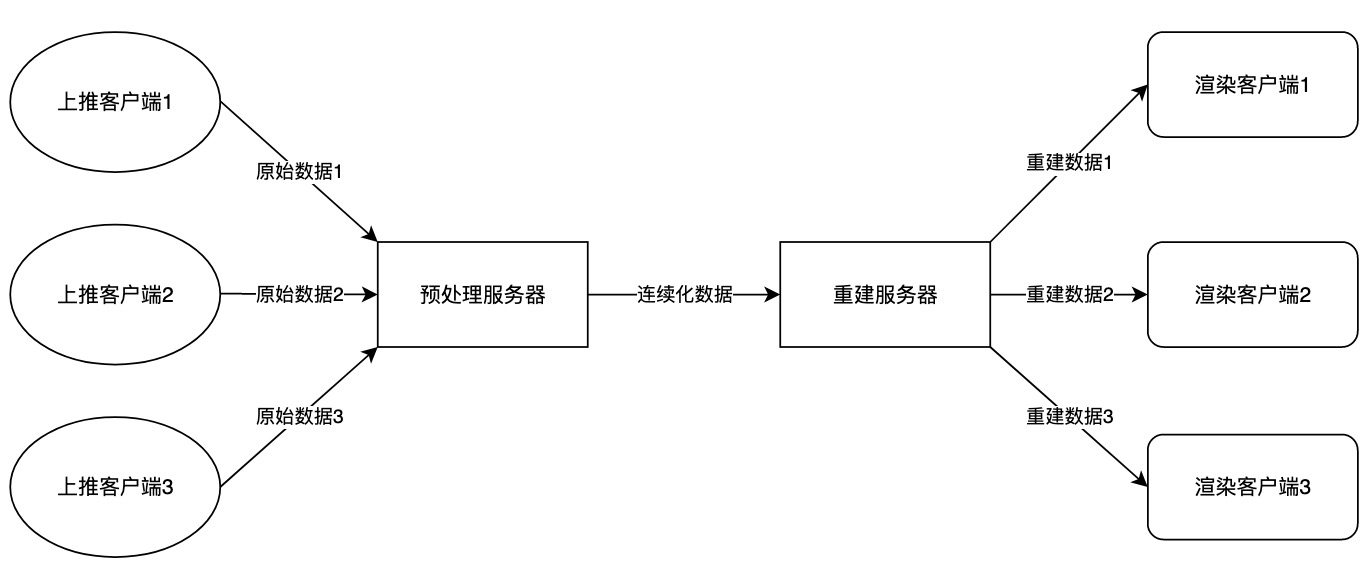
\includegraphics[scale=0.28]{software-structure.png}
\caption{三维可视化软件架构}
\label{fig:software} 
\end{figure}

\FloatBarrier

\subsubsection{数据接口}

原始数据为整个软件的数据入口,由~\ref{sec:ss}节可知FOSS主要感测数据为弯曲曲率,
故本文采用若干个测量点上两个正交方向$a$、$b$的曲率数据为原始数据,其结构如代码块~\ref{lst:raw-data}所示(其中采用的数据表达格式为JSON\cite{rfc7159})。

\begin{lstlisting}[language=json,firstnumber=1,label={lst:raw-data},caption={原始曲率数据样例}]
{
    "ds": 0.01,
    "samples": [
        [0, 0, 0],
        [4.66, 0.21, -0.11],
        [9.36, 0.27, -0.13],
        [14.82, 0.086, -0.21],
        [19.72, -0.0093, 0.08],
        [24.74, -0.091, -0.07],
        [29.95, -0.079, 0],
        ...
    ]
}
\end{lstlisting}

其中$d_s$为建议插值步长,
$samples$数组内的每个元素都是一个三元组,三个数据分别代表距离原点的弧长$s$、$a$方向的曲率$k_a$和$b$方向的曲率$k_b$。

离散的原始数据插值即可得到连续化数据,其结构如代码块~\ref{lst:curvature-vec}所示。

\begin{lstlisting}[language=json,firstnumber=1,label={lst:curvature-vec},caption={插值曲率数据样例}]
{
    "ds": 0.02,
    "ks": [
        [0, 0],
        [0.005, -0.004],
        [0.009, -0.007],
        [0.013, -0.008],
        [0.017, 0.0023],
        [0.022, 0.006],
        [0.025, 0.008],
        [0.031, 0.012],
        [0.033, 0.007],
        [0.03, 0.01],
        ...
    ]
}
\end{lstlisting}

其中$d_s$为实际采用的插值步长,
$ks$数组内的每个元素都是一个二元组,两个数据分别代表$a$方向的曲率$k_a$和$b$方向的曲率$k_b$。

根据连续化数据进行坐标重建即可得到重建数据,其结构如代码块~\ref{lst:positions}所示。

\begin{lstlisting}[language=json,firstnumber=1,label={lst:positions},caption={重建坐标点数据样例}]
{
    "timestamp": 1595915002,
    "points": [
        [0.009999833069741726,1.0000499486923218,0],
        [0.019999666139483452,0.9999996423721313,0],
        [0.029998499900102615,0.9998496174812317,0],
        [0.03999536111950874,0.9996007680892944,0],
        [0.04998929798603058,0.9992536902427673,0],
        [0.059979379177093506,0.998809278011322,0],
        [0.0699646919965744,0.998268187046051,0],
        [0.07994434982538223,0.9976312518119812,0],
        [0.08991748839616776,0.9968992471694946,0],
        [0.09988325089216232,0.9960729479789734,0],
        [0.10984081774950027,0.9951531291007996,0],
        [0.11978939175605774,0.994140625,0],
        [0.009999833069741726,1.0000499486923218,0],
        ...
    ]
}
\end{lstlisting}

其中$timestamp$是数据产生时的时间戳,$points$数组内的每个元素都是一个三元组,
三个数分别是$x$轴、$y$轴和$z$轴的坐标。

\subsubsection{功能指标}
本文可视化软件的主要功能指标有通用性、安全性、准确性和实时性。

其中通用性指客户端是否通用,包括原始数据上推客户端和渲染客户端。原始数据上推客户端的通用性就是上推数据接口的通用性,
即形变传感器的感测数据是否普遍能满足软件的原始数据接口。根据\nameref{sec:ss},原始数据上推客户端的通用性优良。
而渲染客户端的通用性指客户端软件的运行是跨平台的、使用简便的,这需要渲染引擎和程序实现的保证。

安全性指各模块间数据传输是否安全,是否有被冒充、篡改或窃听的风险,需要数据传输协议的保证。

准确性指重建坐标与实际坐标之间的一致程度,重建误差越小,准确性越好,需要重建算法及其实现的保证。

实时性指从原始数据上推到完成渲染整个流程的耗时是否够短。在串行实现(即单帧重建)中实时性直接体现在渲染帧率。
例如单帧渲染时间必须小于16.7ms才能保证60帧率的渲染画面,同时需要网络带宽、延迟和重建算法的保证。

\subsection{本章小结}
本章主要讨论了形变传感器的研究进展,确定了软件的整体架构并提出了软件的功能指标,
但软件的具体构建还需要考虑以下三个问题:

\begin{itemize}
\item 如何通过传感器获取的数据重建出曲线的空间各点坐标?
\item 如何将服务端重建的点坐标安全又实时地传输到客户端渲染程序?
\item 又如何根据各点坐标渲染出三维图形?
\end{itemize}

这些问题将在下一章中讨论。
